\section{エラー率の導入}
GA戦略が結果として最も低い所持金となった原因は、シミュレーションを行う条件にあった。GA戦略は複雑性が低い、つまりシンプルであることが最大の特徴である。そこで、我々はGA戦略の特徴がどのくらい有用かを調べるために複雑性を考慮したシミュレーションを行う必要があった。そして、そのシミュレーションを行うため、複雑性に関する実験の結果をもとにエラー率という概念を作成した。エラー率の定義は、ある戦略を使用する際にプレイヤーが行動を間違えてしまう確率を表したものである。このエラー率をシミュレーションに適用することにより、GA戦略を使用した際のプレイヤーの所持金が良い方向に改善される可能性があるのではないかと考えた。このエラー率の導出方法は、複雑性に関する実験データの正答率を線形回帰分析をエクセルの分析ツールを使用した。また、使用した実験データについては以下の\ref{hoge}で示す通りである。
\begin{table}[H]
\begin{tabular}{lllll}
複雑性&0.2&0.2&0.407&0.448 \\
エラー率&0.002&0.009&0.125&0.162 \\ 
\end{tabular}
\caption{複雑性と誤答率}
\label{hoge}
\end{table}
また、以上の実験データから線形回帰分析により得られた式は、
\begin{equation}
y=0.611x - 0.1172
\end{equation}
となった。この式を横軸を複雑性、縦軸をエラー率としてグラフにしたものが以下の\ref{hoge2}である。
\begin{figure}[H]
\begin{center}
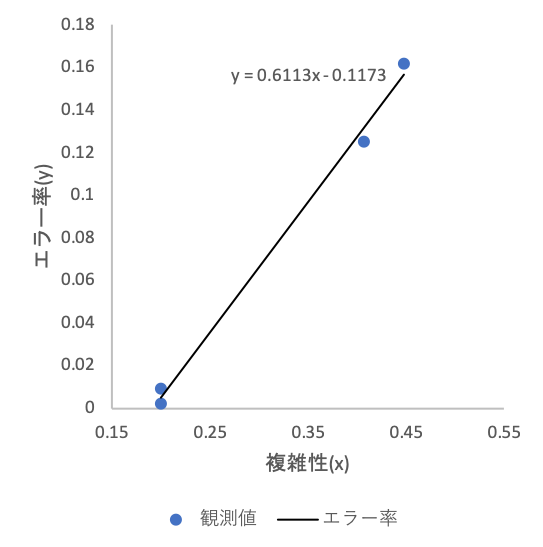
\includegraphics[width=10cm]{figure/error_rate.png}
\caption{線形回帰分析によるエラー率のグラフ}
\end{center}
\end{figure}
\bunseki{*薩田凱斗}